\documentclass[]{article}
\usepackage{lmodern}
\usepackage{amssymb,amsmath}
\usepackage{ifxetex,ifluatex}
\usepackage{fixltx2e} % provides \textsubscript
\ifnum 0\ifxetex 1\fi\ifluatex 1\fi=0 % if pdftex
  \usepackage[T1]{fontenc}
  \usepackage[utf8]{inputenc}
\else % if luatex or xelatex
  \ifxetex
    \usepackage{mathspec}
  \else
    \usepackage{fontspec}
  \fi
  \defaultfontfeatures{Ligatures=TeX,Scale=MatchLowercase}
\fi
% use upquote if available, for straight quotes in verbatim environments
\IfFileExists{upquote.sty}{\usepackage{upquote}}{}
% use microtype if available
\IfFileExists{microtype.sty}{%
\usepackage{microtype}
\UseMicrotypeSet[protrusion]{basicmath} % disable protrusion for tt fonts
}{}
\usepackage[margin=1in]{geometry}
\usepackage{hyperref}
\hypersetup{unicode=true,
            pdftitle={Laborator 6},
            pdfborder={0 0 0},
            breaklinks=true}
\urlstyle{same}  % don't use monospace font for urls
\usepackage{color}
\usepackage{fancyvrb}
\newcommand{\VerbBar}{|}
\newcommand{\VERB}{\Verb[commandchars=\\\{\}]}
\DefineVerbatimEnvironment{Highlighting}{Verbatim}{commandchars=\\\{\}}
% Add ',fontsize=\small' for more characters per line
\usepackage{framed}
\definecolor{shadecolor}{RGB}{248,248,248}
\newenvironment{Shaded}{\begin{snugshade}}{\end{snugshade}}
\newcommand{\KeywordTok}[1]{\textcolor[rgb]{0.13,0.29,0.53}{\textbf{#1}}}
\newcommand{\DataTypeTok}[1]{\textcolor[rgb]{0.13,0.29,0.53}{#1}}
\newcommand{\DecValTok}[1]{\textcolor[rgb]{0.00,0.00,0.81}{#1}}
\newcommand{\BaseNTok}[1]{\textcolor[rgb]{0.00,0.00,0.81}{#1}}
\newcommand{\FloatTok}[1]{\textcolor[rgb]{0.00,0.00,0.81}{#1}}
\newcommand{\ConstantTok}[1]{\textcolor[rgb]{0.00,0.00,0.00}{#1}}
\newcommand{\CharTok}[1]{\textcolor[rgb]{0.31,0.60,0.02}{#1}}
\newcommand{\SpecialCharTok}[1]{\textcolor[rgb]{0.00,0.00,0.00}{#1}}
\newcommand{\StringTok}[1]{\textcolor[rgb]{0.31,0.60,0.02}{#1}}
\newcommand{\VerbatimStringTok}[1]{\textcolor[rgb]{0.31,0.60,0.02}{#1}}
\newcommand{\SpecialStringTok}[1]{\textcolor[rgb]{0.31,0.60,0.02}{#1}}
\newcommand{\ImportTok}[1]{#1}
\newcommand{\CommentTok}[1]{\textcolor[rgb]{0.56,0.35,0.01}{\textit{#1}}}
\newcommand{\DocumentationTok}[1]{\textcolor[rgb]{0.56,0.35,0.01}{\textbf{\textit{#1}}}}
\newcommand{\AnnotationTok}[1]{\textcolor[rgb]{0.56,0.35,0.01}{\textbf{\textit{#1}}}}
\newcommand{\CommentVarTok}[1]{\textcolor[rgb]{0.56,0.35,0.01}{\textbf{\textit{#1}}}}
\newcommand{\OtherTok}[1]{\textcolor[rgb]{0.56,0.35,0.01}{#1}}
\newcommand{\FunctionTok}[1]{\textcolor[rgb]{0.00,0.00,0.00}{#1}}
\newcommand{\VariableTok}[1]{\textcolor[rgb]{0.00,0.00,0.00}{#1}}
\newcommand{\ControlFlowTok}[1]{\textcolor[rgb]{0.13,0.29,0.53}{\textbf{#1}}}
\newcommand{\OperatorTok}[1]{\textcolor[rgb]{0.81,0.36,0.00}{\textbf{#1}}}
\newcommand{\BuiltInTok}[1]{#1}
\newcommand{\ExtensionTok}[1]{#1}
\newcommand{\PreprocessorTok}[1]{\textcolor[rgb]{0.56,0.35,0.01}{\textit{#1}}}
\newcommand{\AttributeTok}[1]{\textcolor[rgb]{0.77,0.63,0.00}{#1}}
\newcommand{\RegionMarkerTok}[1]{#1}
\newcommand{\InformationTok}[1]{\textcolor[rgb]{0.56,0.35,0.01}{\textbf{\textit{#1}}}}
\newcommand{\WarningTok}[1]{\textcolor[rgb]{0.56,0.35,0.01}{\textbf{\textit{#1}}}}
\newcommand{\AlertTok}[1]{\textcolor[rgb]{0.94,0.16,0.16}{#1}}
\newcommand{\ErrorTok}[1]{\textcolor[rgb]{0.64,0.00,0.00}{\textbf{#1}}}
\newcommand{\NormalTok}[1]{#1}
\usepackage{graphicx,grffile}
\makeatletter
\def\maxwidth{\ifdim\Gin@nat@width>\linewidth\linewidth\else\Gin@nat@width\fi}
\def\maxheight{\ifdim\Gin@nat@height>\textheight\textheight\else\Gin@nat@height\fi}
\makeatother
% Scale images if necessary, so that they will not overflow the page
% margins by default, and it is still possible to overwrite the defaults
% using explicit options in \includegraphics[width, height, ...]{}
\setkeys{Gin}{width=\maxwidth,height=\maxheight,keepaspectratio}
\IfFileExists{parskip.sty}{%
\usepackage{parskip}
}{% else
\setlength{\parindent}{0pt}
\setlength{\parskip}{6pt plus 2pt minus 1pt}
}
\setlength{\emergencystretch}{3em}  % prevent overfull lines
\providecommand{\tightlist}{%
  \setlength{\itemsep}{0pt}\setlength{\parskip}{0pt}}
\setcounter{secnumdepth}{5}
% Redefines (sub)paragraphs to behave more like sections
\ifx\paragraph\undefined\else
\let\oldparagraph\paragraph
\renewcommand{\paragraph}[1]{\oldparagraph{#1}\mbox{}}
\fi
\ifx\subparagraph\undefined\else
\let\oldsubparagraph\subparagraph
\renewcommand{\subparagraph}[1]{\oldsubparagraph{#1}\mbox{}}
\fi

%%% Use protect on footnotes to avoid problems with footnotes in titles
\let\rmarkdownfootnote\footnote%
\def\footnote{\protect\rmarkdownfootnote}

%%% Change title format to be more compact
\usepackage{titling}

% Create subtitle command for use in maketitle
\newcommand{\subtitle}[1]{
  \posttitle{
    \begin{center}\large#1\end{center}
    }
}

\setlength{\droptitle}{-2em}
  \title{Laborator 6}
  \pretitle{\vspace{\droptitle}\centering\huge}
  \posttitle{\par}
\subtitle{Elemente de estimare punctuală}
  \author{}
  \preauthor{}\postauthor{}
  \date{}
  \predate{}\postdate{}

\usepackage{booktabs}
\usepackage{longtable}
\usepackage{framed,color}
\definecolor{shadecolor}{RGB}{248, 248, 248}
\definecolor{shadecolor1}{RGB}{216,225,235}
\definecolor{framecolor}{RGB}{108,123,13}

\ifxetex
  \usepackage{letltxmacro}
  \setlength{\XeTeXLinkMargin}{1pt}
  \LetLtxMacro\SavedIncludeGraphics\includegraphics
  \def\includegraphics#1#{% #1 catches optional stuff (star/opt. arg.)
    \IncludeGraphicsAux{#1}%
  }%
  \newcommand*{\IncludeGraphicsAux}[2]{%
    \XeTeXLinkBox{%
      \SavedIncludeGraphics#1{#2}%
    }%
  }%
\fi

\newenvironment{frshaded*}{%
  \def\FrameCommand{\fboxrule=\FrameRule\fboxsep=\FrameSep \fcolorbox{framecolor}{shadecolor1}}%
  \MakeFramed {\advance\hsize-\width \FrameRestore}}%
{\endMakeFramed}

\newenvironment{rmdblock}[1]
  {\begin{frshaded*}
  \begin{itemize}
  \renewcommand{\labelitemi}{
    \raisebox{-.7\height}[0pt][0pt]{
      {\setkeys{Gin}{width=2em,keepaspectratio}\includegraphics{images/icons/#1}}
    }
  }
  \item
  }
  {
  \end{itemize}
  \end{frshaded*}
  }
  
\newenvironment{rmdcaution}
  {\begin{rmdblock}{caution}}
  {\end{rmdblock}}
% \newenvironment{rmdinsight}
%   {\begin{rmdblock}{insight}}
%   {\end{rmdblock}}
\newenvironment{rmdexercise}
  {\begin{rmdblock}{exercise}}
  {\end{rmdblock}}
\newenvironment{rmdtip}
  {\begin{rmdblock}{tip}}
  {\end{rmdblock}}
  
  
%%%%%%%%%%%%%%%%%%%%%%%%%%%%%%%%%%%%%%%%%%%%%%%%%%%%%%%%%%%%%%%%%%%%%%%%%%%%%%%%%%%%%%%%%%%%%%%%%%%%%%%%%%%%%%%%%%%%%
%%%%%%%%%%% For insight block %%%%%%%%%%%%%%%%%%%%%%%%%%
\definecolor{shadecolor_insight}{RGB}{223,240,216}
\definecolor{framecolor_insight}{RGB}{136,193,137}

\newenvironment{frshaded_insight*}{%
  \def\FrameCommand{\fboxrule=\FrameRule\fboxsep=\FrameSep \fcolorbox{framecolor_insight}{shadecolor_insight}}%
  \MakeFramed {\advance\hsize-\width \FrameRestore}}%
{\endMakeFramed}

\newenvironment{rmdblock_insight}[1]
  {\begin{frshaded_insight*}
  \begin{itemize}
  \renewcommand{\labelitemi}{
    \raisebox{-.7\height}[0pt][0pt]{
      {\setkeys{Gin}{width=2em,keepaspectratio}\includegraphics{images/icons/#1}}
    }
  }
  \item
  }
  {
  \end{itemize}
  \end{frshaded_insight*}
  }
  
\newenvironment{rmdinsight}
  {\begin{rmdblock_insight}{insight}}
  {\end{rmdblock_insight}}
  
%%%%%%%%%%%%%%%%%%%%%%%%%%%%%%%%%%%%%%%%%%%%%%%%%%%%%%%%%%%%%%%%%%%%%%%%%%%%%%%%%%%%%%%%%%%%%%%%%%%%%%%%%%%%%%%%%%%%%
\usepackage{subfigure}
\usepackage{booktabs}
\usepackage{slashbox}
\usepackage{color}
%%%%%%%%%%%%%%%%%%%%%%%%%%%%%%%%%%%%%%%%%%%%%%%%%%%%%%%%%%%%%%%%%%%%%%%%%%%%%%%%%%%%%%%%%%%%%%%%%%%%%%%%%%%%%%%%%%%%%
%CITEVA DEFINITII
\def\om{\omega}
\def\Om{\Omega}
\def\et{\eta}
\def\td{\tilde{\delta}}
\def\m{{\mu}}
\def\n{{\nu}}
\def\k{{\kappa}}
\def\l{{\lambda}}
\def\L{{\Lambda}}
\def\g{{\gamma}}
\def\a{{\alpha}}
\def\e{{\varepsilon}}
\def\b{{\beta}}
\def\G{{\Gamma}}
\def\d{{\delta}}
\def\D{{\Delta}}
\def\t{{\theta}}
\def\s{{\sigma}}
\def\S{{\Sigma}}
\def\z{{\zeta}}
\def\qed{\hfill\Box}
\def\ds{\displaystyle}
\def\mc{\mathcal}
%%%%%%%%%%%%%%%%%%%%%%%%%%%%%%%%%%%%%%%%%%%%%%%%%%%%%%%%%%%%%%%%%%%%%%%%%%%%%%%%%%%%%%%%%%%%%%%%%%%%%%%%%%%%%%%%%%%%%%
\def\1{{\mathbf 1}}
\def\CC{{\mathbb C}}
\def\VV{{\mathbb V}}
\def\RR{{\mathbb R}}
\def\QQ{{\mathbb Q}}
\def\ZZ{{\mathbb Z}}
\def\PP{{\mathbb P}}
\def\EE{{\mathbb E}}
\def\NN{{\mathbb N}}
\def\FF{{\mathbb F}}
%\def\SS{{\mathbb S}}
\def\MA{{\mathcal A}}
\def\MO{{\mathcal O}}
\def\MF{{\mathcal F}}
\def\ME{{\mathcal E}}
\def\MR{{\mathcal R}}
\def\MB{{\mathcal B}}
\def\MM{{\mathcal M}}
\def\MN{{\mathcal N}}
\def\MU{{\mathcal U}}
\def\MP{{\mathcal P}}
\def\MS{{\mathcal S}}
\def\MBS{{\mathbf S}}
\def\MX{{\bm{ \mathscr X}}}

% independent sign
\newcommand\independent{\protect\mathpalette{\protect\independenT}{\perp}}
\def\independenT#1#2{\mathrel{\rlap{$#1#2$}\mkern2mu{#1#2}}}

\renewcommand{\figurename}{Fig.}

%%%%%%%%%%%%%%%%%%%%%%%%%%%%%%%%%%%%%%%%%%%%%%%%%%%%%%%%%%%%%%%%%%%%%%%%%%%%%%%%%%%%%%%%%%%%%%%%%%%%%%%%%%%%%%%%%%%%%
%Header and Footer
\usepackage{fancyhdr}

\pagestyle{fancy}
\fancyhf{}
\rhead{Universitatea din Bucure\c sti\\ Facultatea de Matematic\u a \c si Informatic\u a}
\lhead{\textit{Curs}: Statistic\u a\\ \textit{Instructori}: A. Am\u arioarei, S. Cojocea}
\rfoot{Pagina \thepage}
\lfoot{Grupele: 301, 311, 321}
%%%%%%%%%%%%%%%%%%%%%%%%%%%%%%%%%%%%%%%
\usepackage{booktabs}
\usepackage{longtable}
\usepackage{array}
\usepackage{multirow}
\usepackage[table]{xcolor}
\usepackage{wrapfig}
\usepackage{float}
\usepackage{colortbl}
\usepackage{pdflscape}
\usepackage{tabu}
\usepackage{threeparttable}

\begin{document}
\maketitle

%%%%%%%%%%%%%%%%%%%%%%%%
\thispagestyle{fancy}

Obiectivul acestui laborator este de a ilustra noțiunea de consistență a
unui estimator precum și de a compara mai mulți estimatori.

\section{Proprietăți ale
estimatorilor}\label{proprietati-ale-estimatorilor}

\subsection{Exemplu de comparare a trei
estimatori}\label{exemplu-de-comparare-a-trei-estimatori}

\begin{rmdexercise}
Fie \(X_1,X_2,\ldots,X_n\) un eșantion de talie \(n\) dintr-o populație
normală de medie \(\mu\) și varianță \(\sigma^2\). Atunci

\[
  \hat{\mu}_1 = \frac{1}{n}\sum_{i=1}^{n}X_i, \quad \hat{\mu}_2 = M_n\,(\text{mediana}\,), \quad \hat{\mu}_3 = \frac{X_{(1)} + X_{(n)}}{2}
\]

sunt trei estimatori punctuali pentru \(\mu\). Creați o funcție care să
ilustreze cum sunt repartizați cei trei estimatori. Începeți cu
\(n = 10\), \(\mu = 0\) și \(\sigma^2 = 1\) și trasați histogramele
pentru a-i compara. Ce se întâmplă dacă schimbați \(n\), \(\mu\) sau
\(\sigma^2\) ?
\end{rmdexercise}

Vom crea o funcție numită \texttt{norm\_estimators} care va construi
repartițiile celor trei estimatori:

\begin{Shaded}
\begin{Highlighting}[]
\NormalTok{norm_estimators =}\StringTok{ }\ControlFlowTok{function}\NormalTok{(n, mu, sigma, S)\{}
  \CommentTok{# Initializam}
\NormalTok{  mu1 =}\StringTok{ }\KeywordTok{numeric}\NormalTok{(S)}
\NormalTok{  mu2 =}\StringTok{ }\KeywordTok{numeric}\NormalTok{(S)}
\NormalTok{  mu3 =}\StringTok{ }\KeywordTok{numeric}\NormalTok{(S)}
  
  \CommentTok{# repetam experimentul de S ori}
  \ControlFlowTok{for}\NormalTok{ (i }\ControlFlowTok{in} \DecValTok{1}\OperatorTok{:}\NormalTok{S)\{}
\NormalTok{    x =}\StringTok{ }\KeywordTok{rnorm}\NormalTok{(n, }\DataTypeTok{mean =}\NormalTok{ mu, }\DataTypeTok{sd =}\NormalTok{ sigma)}
    
    \CommentTok{# calculam estimatorii}
\NormalTok{    mu1[i] =}\StringTok{ }\KeywordTok{mean}\NormalTok{(x)}
\NormalTok{    mu2[i] =}\StringTok{ }\KeywordTok{median}\NormalTok{(x)}
\NormalTok{    mu3[i] =}\StringTok{ }\NormalTok{(}\KeywordTok{min}\NormalTok{(x)}\OperatorTok{+}\KeywordTok{max}\NormalTok{(x))}\OperatorTok{/}\DecValTok{2}
\NormalTok{  \}}
  
  \CommentTok{# afisam variantele estimatorilor }
  \KeywordTok{print}\NormalTok{(}\KeywordTok{cbind}\NormalTok{(}\DataTypeTok{var_mu1 =} \KeywordTok{var}\NormalTok{(mu1), }\DataTypeTok{var_mu2 =} \KeywordTok{var}\NormalTok{(mu2), }\DataTypeTok{var_mu3 =} \KeywordTok{var}\NormalTok{(mu3)))}
  
 \KeywordTok{return}\NormalTok{(}\KeywordTok{cbind}\NormalTok{(}\DataTypeTok{mu1 =}\NormalTok{ mu1, }\DataTypeTok{mu2 =}\NormalTok{ mu2, }\DataTypeTok{mu3 =}\NormalTok{ mu3))}
  
\NormalTok{\}}
\end{Highlighting}
\end{Shaded}

Pentru a ilustra grafic histogramele celor trei estimatori, considerăm
\(\mu = 0\) și \(\sigma^2 = 1\) și avem:

\begin{verbatim}
         var_mu1     var_mu2    var_mu3
[1,] 0.001004297 0.001616957 0.06173788
\end{verbatim}

\begin{center}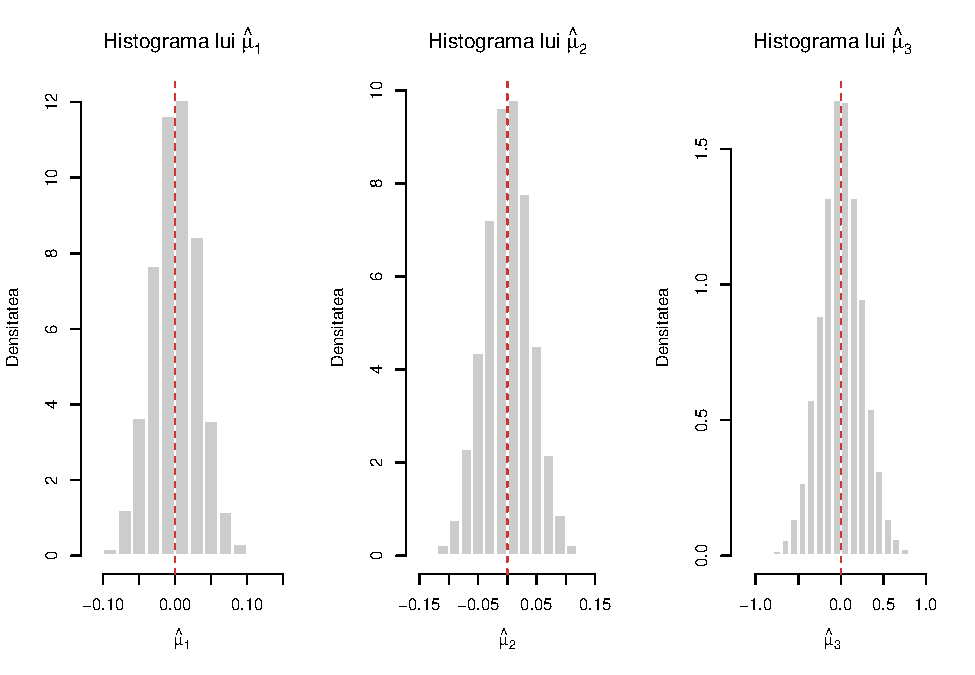
\includegraphics[width=0.7\linewidth]{Lab_6_files/figure-latex/unnamed-chunk-4-1} \end{center}

\subsection{Ilustrarea consistenței unui
estimator}\label{ilustrarea-consistentei-unui-estimator}

\begin{rmdexercise}
Fie \(X_1,X_2,\ldots,X_n\) un eșantion de talie \(n\) dintr-o populație
\(Pois(\theta)\). Ilustrați grafic consistența estimatorului
\(\hat{\theta}_n = S_n^2\) trasând histograma repartiției lui
\(\hat{\theta}_n\) pentru \(n\in\{10,25,50,100\}\). Ce observați?
\end{rmdexercise}

Considerăm funcția \texttt{pois\_est} care pentru \(\theta\) fixat
simulează repartiția estimatorului \(\hat{\theta}_n\):

\begin{Shaded}
\begin{Highlighting}[]
\NormalTok{pois_est1 =}\StringTok{ }\ControlFlowTok{function}\NormalTok{(n, theta, S)\{}
  \CommentTok{# initializare}
\NormalTok{  sigma1 =}\StringTok{ }\KeywordTok{numeric}\NormalTok{(S)}
  
  \ControlFlowTok{for}\NormalTok{ (i }\ControlFlowTok{in} \DecValTok{1}\OperatorTok{:}\NormalTok{S)\{}
\NormalTok{    x =}\StringTok{ }\KeywordTok{rpois}\NormalTok{(n, theta)}
\NormalTok{    sigma1[i] =}\StringTok{ }\KeywordTok{var}\NormalTok{(x)}
\NormalTok{  \}}
  \CommentTok{# afisam varianta estimatorului}
  \KeywordTok{print}\NormalTok{(}\KeywordTok{paste0}\NormalTok{(}\StringTok{"Pentru n = "}\NormalTok{, n,}\StringTok{" varianta estimatorului este "}\NormalTok{, }\KeywordTok{var}\NormalTok{(sigma1)))}
  \KeywordTok{return}\NormalTok{(sigma1)}
\NormalTok{\}}
\end{Highlighting}
\end{Shaded}

Considerând \(\theta = 3\) și \(n\in\{10,25,50,100\}\) avem:

\begin{verbatim}
[1] "Pentru n = 10 varianta estimatorului este 2.36640535383542"
[1] "Pentru n = 25 varianta estimatorului este 0.867491312476916"
[1] "Pentru n = 50 varianta estimatorului este 0.423889651410313"
[1] "Pentru n = 100 varianta estimatorului este 0.209445339803901"
\end{verbatim}

\begin{center}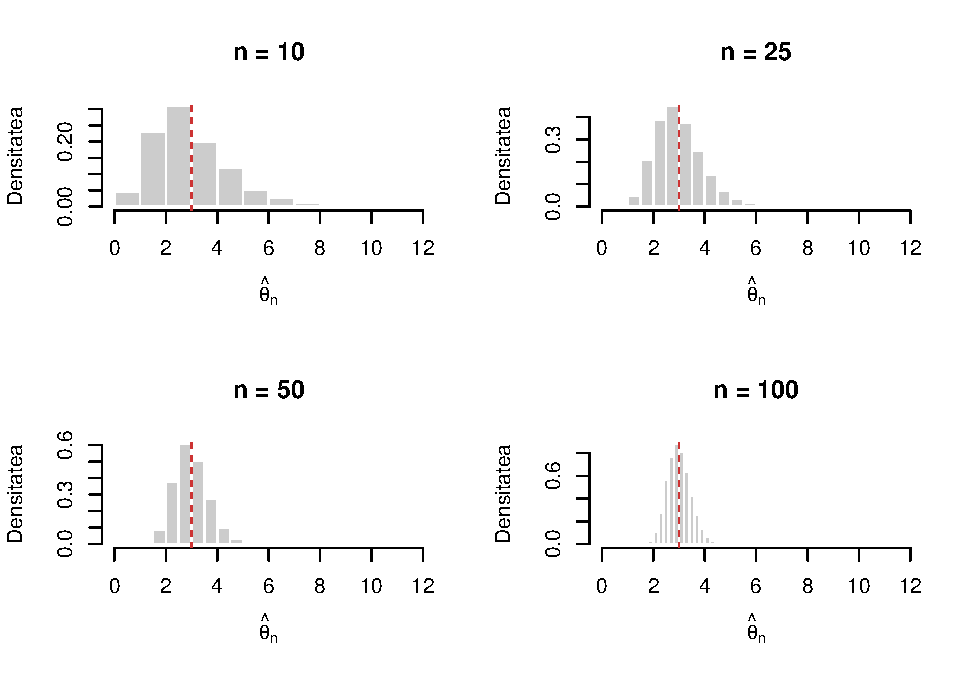
\includegraphics[width=0.7\linewidth]{Lab_6_files/figure-latex/unnamed-chunk-7-1} \end{center}

Ce se întâmplă dacă în loc de \(\hat{\theta}_n\) considerăm estimatorul
\(\tilde{\theta}_n = \bar{X}_n\) sau estimatorul
\(\dot{\theta}_n = \sqrt{\bar{X}_n S_n^2}\) ?

Pentru \(\tilde{\theta}_n\) avem

\begin{verbatim}
[1] "Pentru n = 10 varianta estimatorului este 0.298847741178824"
[1] "Pentru n = 25 varianta estimatorului este 0.120073798790536"
[1] "Pentru n = 50 varianta estimatorului este 0.059625419400548"
[1] "Pentru n = 100 varianta estimatorului este 0.030382726300286"
\end{verbatim}

\begin{center}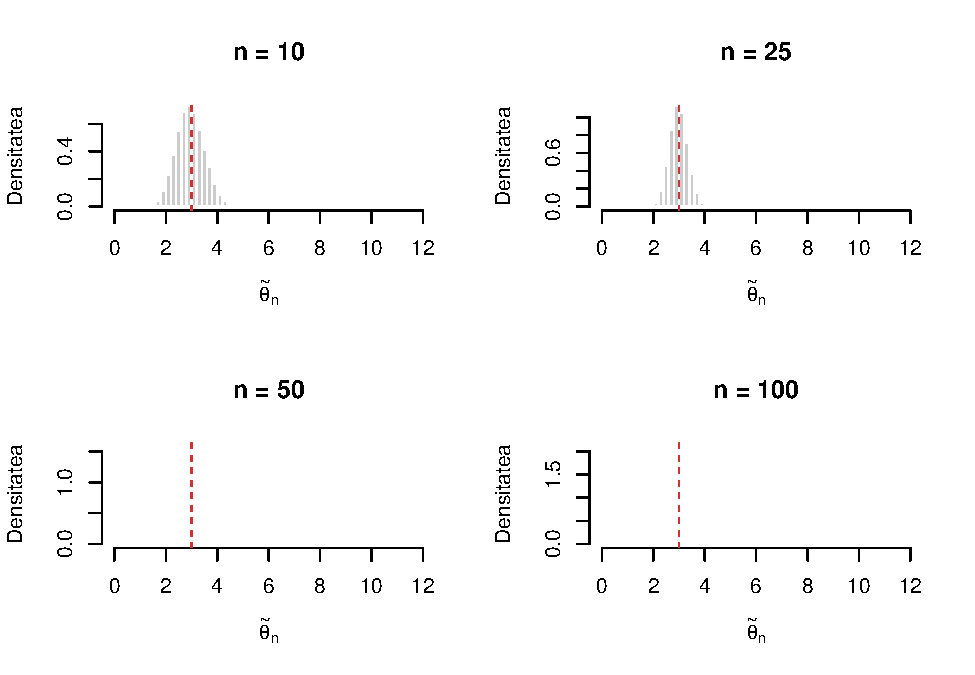
\includegraphics[width=0.7\linewidth]{Lab_6_files/figure-latex/unnamed-chunk-8-1} \end{center}

iar pentru \(\dot{\theta}_n\) avem

\begin{verbatim}
[1] "Pentru n = 10 varianta estimatorului este 0.768686527564423"
[1] "Pentru n = 25 varianta estimatorului este 0.298405855235567"
[1] "Pentru n = 50 varianta estimatorului este 0.148305598496592"
[1] "Pentru n = 100 varianta estimatorului este 0.0749605083080048"
\end{verbatim}

\begin{center}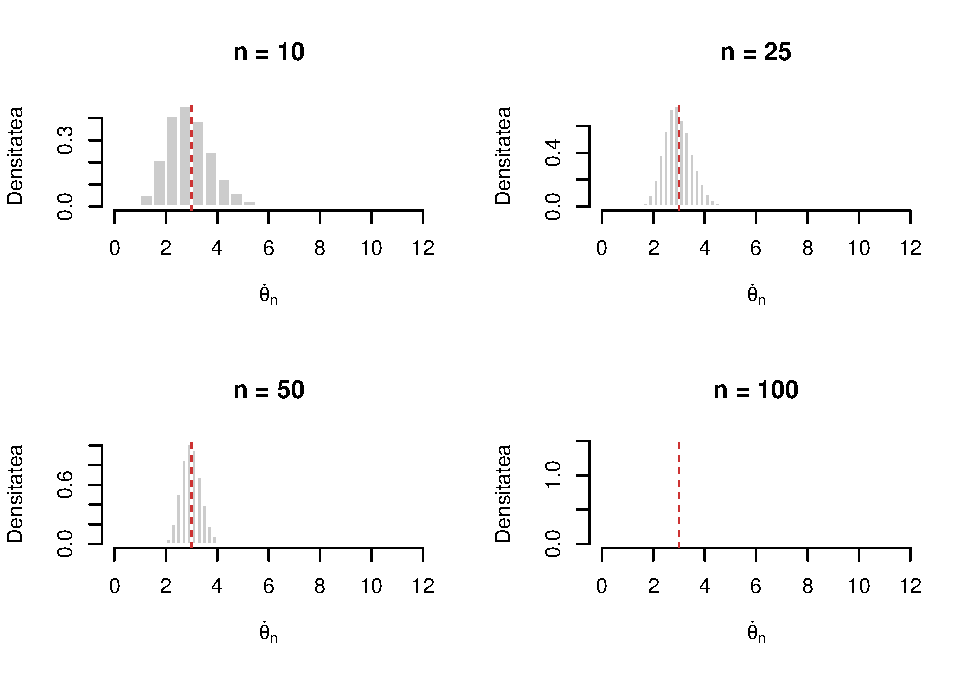
\includegraphics[width=0.7\linewidth]{Lab_6_files/figure-latex/unnamed-chunk-9-1} \end{center}

\section{Estimare prin metoda verosimilității
maxime}\label{estimare-prin-metoda-verosimilitatii-maxime}

\subsection{\texorpdfstring{Exemplu: EVM nu este întotdeauna media
eșantionului chiar dacă
\(\mathbb{E}_{\theta}[\hat{\theta}_n] = \theta\)}{Exemplu: EVM nu este întotdeauna media eșantionului chiar dacă \textbackslash{}mathbb\{E\}\_\{\textbackslash{}theta\}{[}\textbackslash{}hat\{\textbackslash{}theta\}\_n{]} = \textbackslash{}theta}}\label{exemplu-evm-nu-este-intotdeauna-media-esantionului-chiar-daca-mathbbe_thetahattheta_n-theta}

\begin{rmdexercise}
Fie \(X_1,X_2,\ldots,X_n\) un eșantion de talie \(n\) dintr-o populație
Laplace \(L(\theta, c)\) a cărei densitate este dată de formula

\[
  f_{\theta, c}(x) = \frac{1}{2c}e^{-\frac{|x-\theta|}{c}}, \quad -\infty<x<\infty
\]

\begin{enumerate}
\def\labelenumi{\alph{enumi})}
\item
  Ilustrați grafic densitatea și funcția de repartiție a repartiției
  Laplace pentru diferite valori ale parametrilor \(\theta\) (de
  locație) și \(c\) (de scală), e.g. \(\theta\in\{0, 3\}\) și
  \(c\in\{1,2,3,4\}\).
\item
  Determinați estimatorul de verosimilitate maximă \(\hat{\theta}_n\)
  pentru \(\theta\).
\end{enumerate}
\end{rmdexercise}

\begin{enumerate}
\def\labelenumi{\alph{enumi})}
\tightlist
\item
  Se poate arăta cu ușurință că funcția de repartiție a repartiției
  Laplace \(L(\theta, c)\) este
\end{enumerate}

\[
  F_{\theta, c}(x) = \frac{1}{2} + \frac{1}{2}\operatorname{sgn}(x-\theta)\left(1-e^{-\frac{|x-\theta|}{c}}\right) = \left\{\begin{array}{ll}
    \frac{1}{2}e^{-\frac{|x-\theta|}{c}}, & x<\theta\\
    1-\frac{1}{2}e^{-\frac{|x-\theta|}{c}}, & x\geq\theta
  \end{array}\right.
\]

Ilustrarea grafică a densității și a funcției de repartiție pentru
repartiția Laplace:

\begin{center}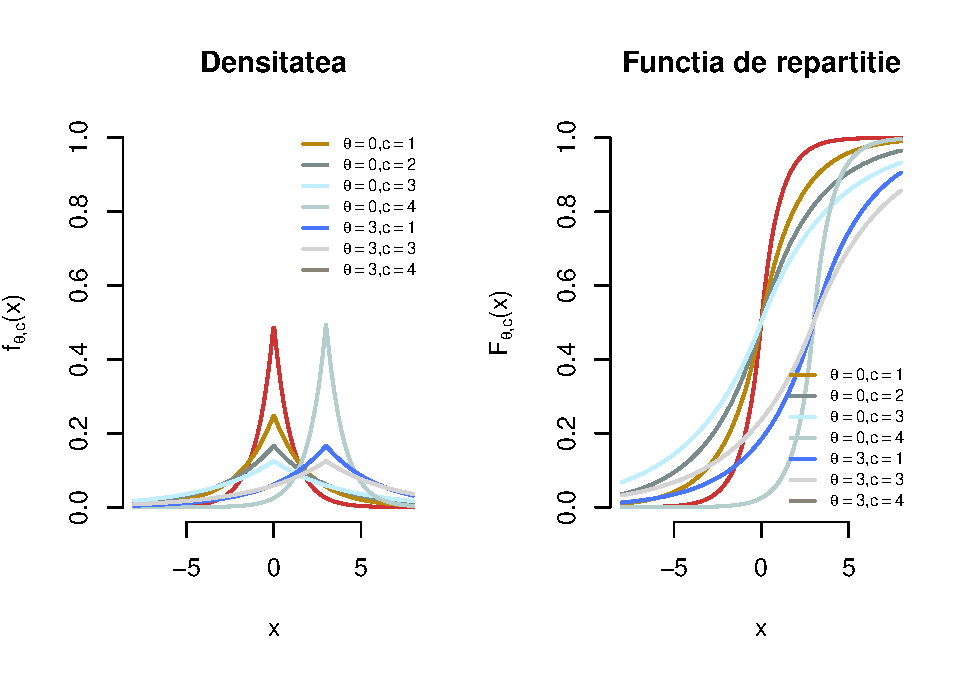
\includegraphics[width=0.7\linewidth]{Lab_6_files/figure-latex/unnamed-chunk-11-1} \end{center}

\begin{enumerate}
\def\labelenumi{\alph{enumi})}
\setcounter{enumi}{1}
\tightlist
\item
  Pentru a determina estimatorul de verosimilitate maximă să observăm că
  funcția de verosimilitate este
\end{enumerate}

\[
L(\theta|\mathbf{X}) = \prod_{i=1}^{n}\left(\frac{1}{2c}e^{-\frac{|X_i-\theta|}{c}}\right) = \frac{1}{(2c)^n}e^{-\sum_{i=1}^{n}\frac{|X_i-\theta|}{c}}
\]

și acesta ia valoarea maximă pentru toate valorile lui \(\theta\) care
minimizează funcția de la exponent

\[
  M(\theta) = \sum_{i=1}^{n}|X_i-\theta| = \sum_{i=1}^{n}|X_{(i)}-\theta|,
\]

unde \(x_{(i)}\) este statistica de ordine de rang \(i\). Se poate vedea
că funcția \(M(\theta)\) este continuă și afină pe porțiuni din figura
de mai jos (pentru un eșantion de talie \(10\) dintr-o populație
\(L(3,1)\) - creați o funcție care vă permite să generați observații
repartizate Laplace).

\begin{center}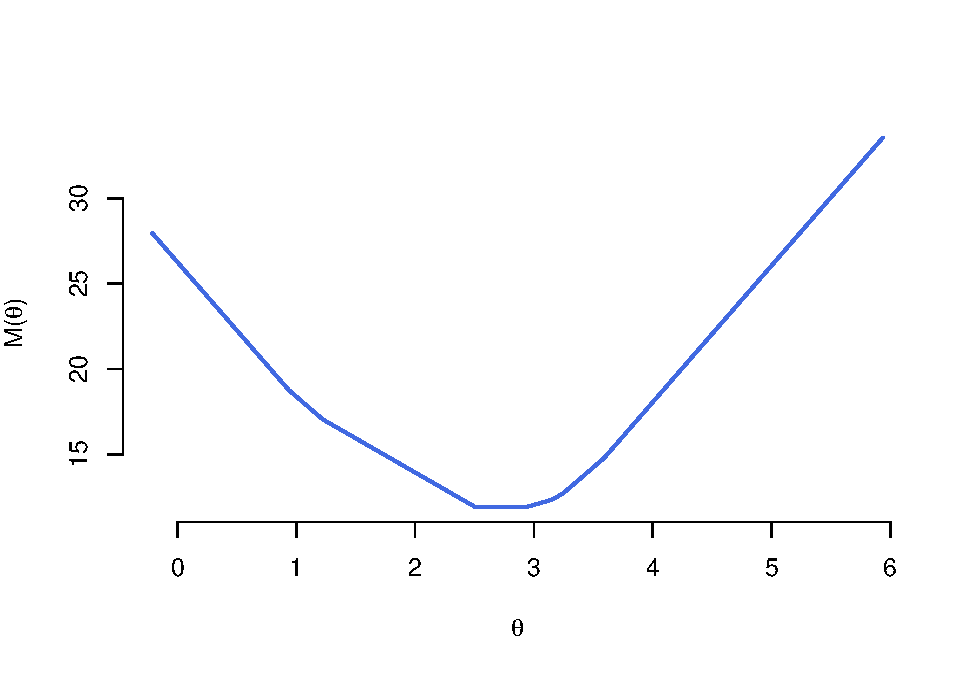
\includegraphics[width=0.7\linewidth]{Lab_6_files/figure-latex/unnamed-chunk-12-1} \end{center}

Observăm că dacă \(\theta\) se află între statistica de ordine de rang
\(m\) și cea de rang \(m+1\), i.e. \(X_{(m)}\leq \theta\leq X_{(m+1)}\),
atunci am avea că \(X_{(i)} \leq X_{(m)} \leq \theta\) dacă \(i\leq m\)
și \(\theta\leq X_{(m+1)}\leq X_{(i)}\) dacă \(m+1\leq i\leq n\), prin
urmare

\[
M(\theta) = \sum_{i=1}^{n}|X_{(i)}-\theta| = \sum_{i=1}^{m}(\theta - X_{(i)}) + \sum_{i=m+1}^{n}(X_{(i)}-\theta)
\]

deci dacă \(X_{(m)}< \theta< X_{(m+1)}\) atunci

\[
\frac{d}{d\theta}M(\theta) = m - (n-m) = 2m-n.
\]

Astfel, \(M'(\theta)<0\) (și \(M(\theta)\) este descrescătoare) dacă
\(m<\frac{n}{2}\) și \(M'(\theta)>0\) (și \(M(\theta)\) este
crescătoare) dacă \(m>\frac{n}{2}\). Dacă \(n = 2k+1\) este impar,
atunci \(\frac{n}{2} = k +\frac{1}{2}\) iar \(M(\theta)\) este strict
descrescătoare dacă \(\theta<X_{(k+1)}\) și strict crescătoare dacă
\(\theta>X_{(k+1)}\) de unde deducem că minimul se atinge pentru
\(\theta = X_{(k+1)}\).

Dacă \(n = 2k\) este par atunci, raționând asemănător, deducem că
\(M(\theta)\) este minimizată pentru orice punct din intervalul
\((X_{(k)}, X_{(k+1)})\), deci orice punct din acest interval va
maximiza și funcția de verosimilitate. Prin convenție alegem estimatorul
de verosimilitate maximă să fie mijlocul acestui interval, i.e.
\(\theta = \frac{X_{(k)} + X_{(k+1)}}{2}\).

Prin urmare am găsit că estimatorul de verosimilitate maximă este
mediana eșantionului

\[
\hat{\theta}_n = \left\{\begin{array}{ll}
  X_{\left(\frac{n+1}{2}\right)}, & \text{$n$ impar}\\
  \frac{X_{\left(\frac{n}{2}\right)} + X_{\left(\frac{n}{2}+1\right)}}{2}, & \text{$n$ par}\\
\end{array}\right.
\]

Mai jos avem ilustrat logaritmul funcției de verosimilitate pentru un
eșantion de volum par (stânga) și unul de volum impar (dreapta):

\begin{center}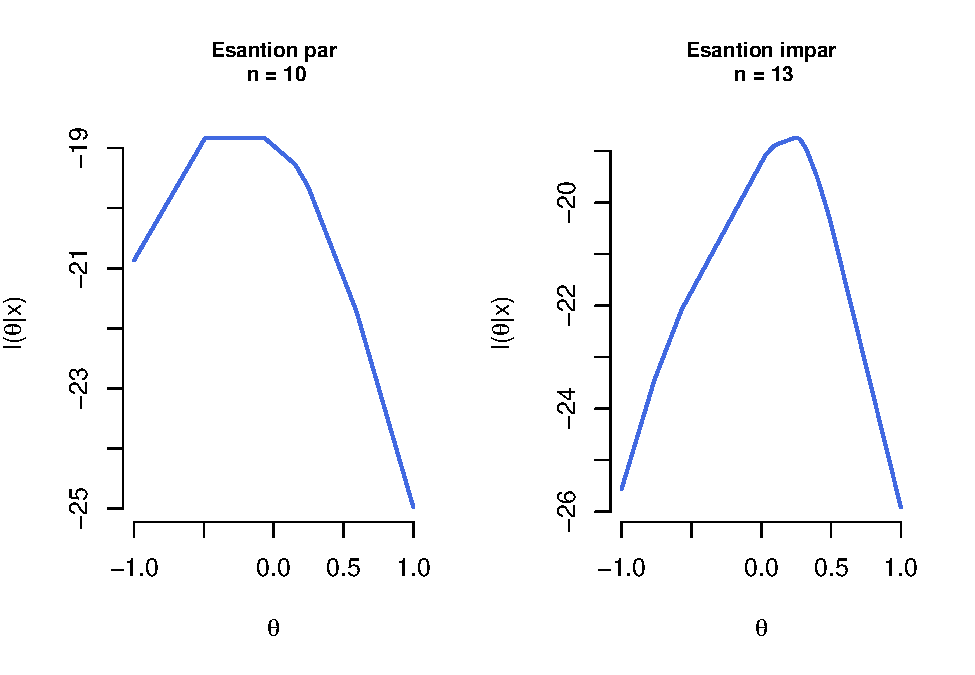
\includegraphics[width=0.7\linewidth]{Lab_6_files/figure-latex/unnamed-chunk-13-1} \end{center}

\subsection{Exemplu de EVM determinat prin soluții
numerice}\label{exemplu-de-evm-determinat-prin-solutii-numerice}

\begin{rmdexercise}
Fie \(X_1,X_2,\ldots,X_n\) un eșantion de talie \(n\) dintr-o populație
logistică a cărei densitate este dată de formula

\[
  f_{\theta}(x) = \frac{e^{-(x-\theta)}}{\left(1+e^{-(x-\theta)}\right)^2}, \quad x\in\mathbb{R},\, \theta\in\mathbb{R} 
\]

Determinați estimatorul de verosimilitate maximă \(\hat{\theta}_n\)
pentru \(\theta\).
\end{rmdexercise}

Densitatea de repartiție și funcția de repartiție a repartiției
logistice sunt ilustrate mai jos (în R se folosesc funcțiile:
\texttt{rlogis}, \texttt{dlogis}, \texttt{plogis} și respectiv
\texttt{qlogis}):

\begin{center}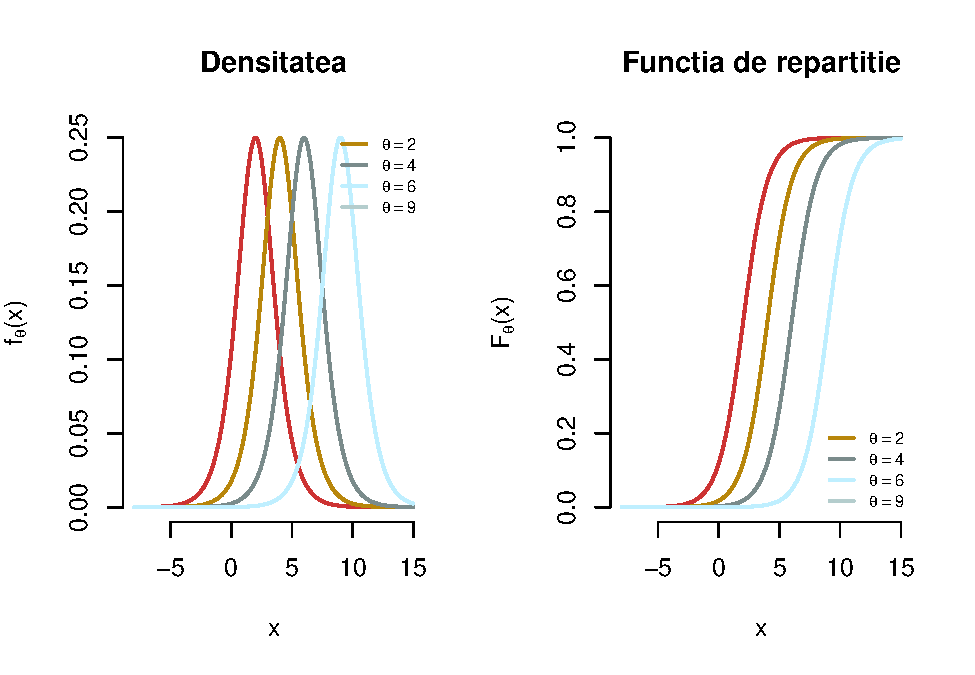
\includegraphics[width=0.7\linewidth]{Lab_6_files/figure-latex/unnamed-chunk-15-1} \end{center}

Observăm că funcția de verosimilitate este dată de

\[
L(\theta|\mathbf{x}) = \prod_{i=1}^{n}f_{\theta}(x_i) = \prod_{i=1}^{n}\frac{e^{-(x_i-\theta)}}{\left(1+e^{-(x_i-\theta)}\right)^2}
\]

iar logaritmul funcției de verosimilitate este

\[
l(\theta|\mathbf{x}) = \sum_{i=1}^{n}\log{f_{\theta}(x_i)} = n\theta - n\bar{x}_n - 2\sum_{i=1}^{n}\log{\left(1+e^{-(x_i-\theta)}\right)}.
\]

Pentru a găsi valoarea lui \(\theta\) care maximizează logaritmul
funcției de verosimilitate și prin urmare a funcției de verosimilitate
trebuie să rezolvăm ecuația \(l'(\theta|\mathbf{x}) = 0\), unde derivata
lui \(l(\theta|\mathbf{x})\) este

\[
l'(\theta|\mathbf{x}) = n - 2\sum_{i = 1}^{n}\frac{e^{-(x_i-\theta)}}{1+e^{-(x_i-\theta)}}
\]

ceea ce conduce la ecuația

\[
  \sum_{i = 1}^{n}\frac{e^{-(x_i-\theta)}}{1+e^{-(x_i-\theta)}} = \frac{n}{2} \tag{$\star$}
\]

Chiar dacă această ecuație nu se simplifică, se poate arăta că această
ecuația admite soluție unică. Observăm că derivata parțiala a membrului
drept în (\(\star\)) devine

\[
\frac{\partial }{\partial \theta}\sum_{i = 1}^{n}\frac{e^{-(x_i-\theta)}}{1+e^{-(x_i-\theta)}} = \sum_{i = 1}^{n}\frac{e^{-(x_i-\theta)}}{\left(1+e^{-(x_i-\theta)}\right)^2}>0
\]

ceea ce arată că membrul stâng este o funcție strict crescătoare în
\(\theta\). Cum membrul stâng în (\(\star\)) tinde spre \(0\) atunci
când \(\theta\to-\infty\) și spre \(n\) pentru \(\theta\to\infty\)
deducem că ecuația (\(\star\)) admite soluție unică (vezi graficul de
mai jos).

\begin{center}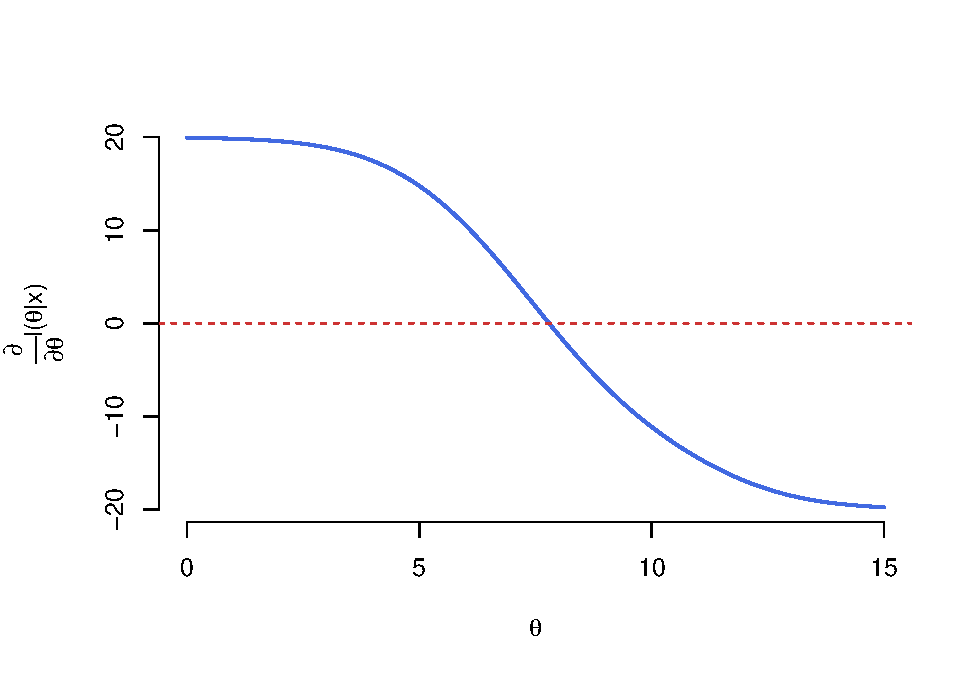
\includegraphics[width=0.7\linewidth]{Lab_6_files/figure-latex/unnamed-chunk-16-1} \end{center}

Cum nu putem găsi o soluție a ecuației \(l'(\theta|\mathbb{x}) = 0\) sub
formă compactă, este necesar să apelăm la metode numerice. O astfel de
metodă numerică este binecunoscuta
\href{https://en.wikipedia.org/wiki/Newton\%27s_method}{metodă a lui
Newton-Raphson}. Metoda presupune să începem cu o valoare (soluție)
inițială \(\hat{\theta}^{(0)}\) și să alegem, plecând de la aceasta, o
nouă valoare \(\hat{\theta}^{(1)}\) definită prin

\[
  \hat{\theta}^{(1)} = \hat{\theta}^{(0)} - \frac{l'\left(\hat{\theta}^{(0)}\right)}{l''\left(\hat{\theta}^{(0)}\right)},
\]

adică \(\hat{\theta}^{(1)}\) este intersecția cu axa absciselor a
tangentei în punctul
\(\left(\hat{\theta}^{(0)}, l'\left(\hat{\theta}^{(0)}\right)\right)\)
la graficul funcției \(l'(\theta)\). Ideea este de a itera procesul până
când soluția converge, cu alte cuvinte pornind de la o valoare
\emph{rezonabilă} de start \(\hat{\theta}^{(0)}\) la pasul \(k+1\) avem

\[
  \hat{\theta}^{(k+1)} = \hat{\theta}^{(k)} - \frac{l'\left(\hat{\theta}^{(k)}\right)}{l''\left(\hat{\theta}^{(k)}\right)}
\]

și oprim procesul atunco când \(k\) este suficient de mare și/sau
\(\left|\hat{\theta}^{(k+1)} - \hat{\theta}^{(k)}\right|\) este
suficient de mic. Următorul grafic ilustrează grafic algoritmul lui
Newton:

\begin{center}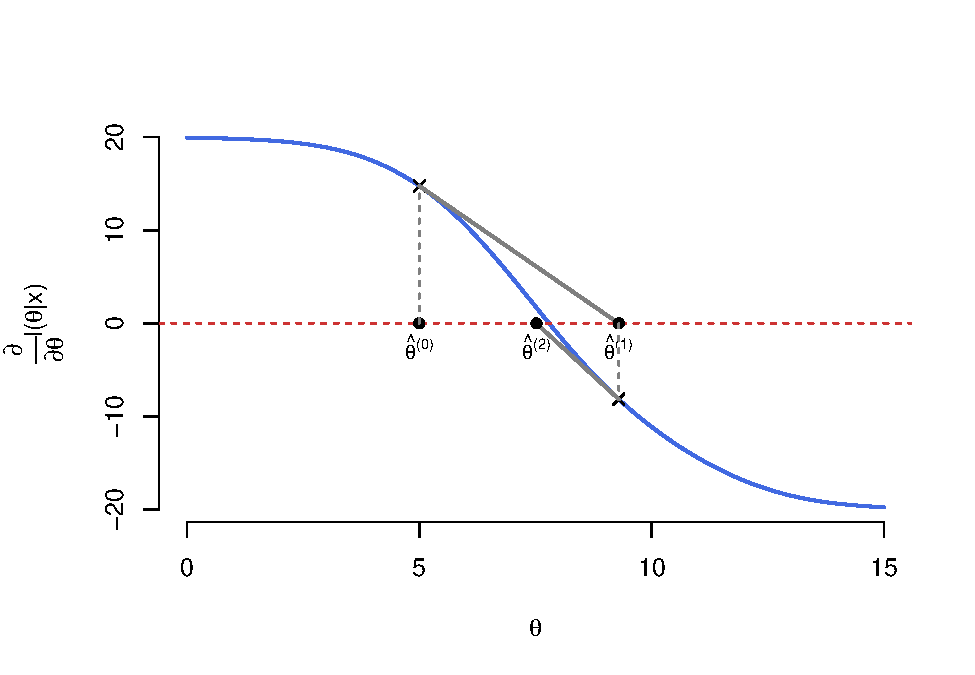
\includegraphics[width=0.7\linewidth]{Lab_6_files/figure-latex/unnamed-chunk-17-1} \end{center}

\textbf{Obs:} Singurul lucru care se schimbă atunci când trecem de la
scalar la vector, este funcția \(l(\theta)\) care acum este o funcție de
\(p>1\) variabile,
\(\theta = (\theta_1, \theta_2, \ldots, \theta_p)^{\intercal}\in\mathbb{R}^p\).
În acest context \(l'(\theta)\) este un vector de derivate parțiale iar
\(l''(\theta)\) este o matrice de derivate parțiale de ordin doi. Prin
urmare itarațiile din metoda lui Newton sunt

\[
  \hat{\theta}^{(k+1)} = \hat{\theta}^{(k)} - \left[l''\left(\hat{\theta}^{(k)}\right)\right]^{-1}l'\left(\hat{\theta}^{(k)}\right)
\] unde \([\cdot]^{-1}\) este
\href{https://en.wikipedia.org/wiki/Moore\%E2\%80\%93Penrose_inverse}{pseudoinversa}
unei matrici.

Funcția de mai jos implementează metoada lui Newton pentru cazul
multidimensional:

\begin{Shaded}
\begin{Highlighting}[]
\CommentTok{# Metoda lui Newton}

\NormalTok{newton <-}\StringTok{ }\ControlFlowTok{function}\NormalTok{(f, df, x0, }\DataTypeTok{eps=}\FloatTok{1e-08}\NormalTok{, }\DataTypeTok{maxiter=}\DecValTok{1000}\NormalTok{, ...) \{}
  \CommentTok{# in caz ca nu e incarcat pachetul sa putem accesa pseudoinversa}
  \ControlFlowTok{if}\NormalTok{(}\OperatorTok{!}\KeywordTok{exists}\NormalTok{(}\StringTok{"ginv"}\NormalTok{)) }\KeywordTok{library}\NormalTok{(MASS) }
  
\NormalTok{  x <-}\StringTok{ }\NormalTok{x0}
\NormalTok{  k <-}\StringTok{ }\DecValTok{0}
  
  \ControlFlowTok{repeat}\NormalTok{ \{}
\NormalTok{    k <-}\StringTok{ }\NormalTok{k }\OperatorTok{+}\StringTok{ }\DecValTok{1}
    
\NormalTok{    x.new <-}\StringTok{ }\NormalTok{x }\OperatorTok{-}\StringTok{ }\KeywordTok{as.numeric}\NormalTok{(}\KeywordTok{ginv}\NormalTok{(}\KeywordTok{df}\NormalTok{(x, ...)) }\OperatorTok\StringTok{ }\KeywordTok{f}\NormalTok{(x, ...))}
    
    \ControlFlowTok{if}\NormalTok{(}\KeywordTok{mean}\NormalTok{(}\KeywordTok{abs}\NormalTok{(x.new }\OperatorTok{-}\StringTok{ }\NormalTok{x)) }\OperatorTok{<}\StringTok{ }\NormalTok{eps }\OperatorTok{|}\StringTok{ }\NormalTok{k }\OperatorTok{>=}\StringTok{ }\NormalTok{maxiter) \{}
      \ControlFlowTok{if}\NormalTok{(k }\OperatorTok{>=}\StringTok{ }\NormalTok{maxiter) }\KeywordTok{warning}\NormalTok{(}\StringTok{"S-a atins numarul maxim de iteratii!"}\NormalTok{)}
      \ControlFlowTok{break}
\NormalTok{    \}}
\NormalTok{    x <-}\StringTok{ }\NormalTok{x.new}
\NormalTok{  \}}
\NormalTok{  out <-}\StringTok{ }\KeywordTok{list}\NormalTok{(}\DataTypeTok{solution =}\NormalTok{ x.new, }\DataTypeTok{value =} \KeywordTok{f}\NormalTok{(x.new, ...), }\DataTypeTok{iter =}\NormalTok{ k)}
  
  \KeywordTok{return}\NormalTok{(out)}
\NormalTok{\}}
\end{Highlighting}
\end{Shaded}

Să presupunem că am observat următorul eșantion de talie \(20\) din
repartiția logistică:

\begin{verbatim}
 [1]  6.996304  9.970107 12.304991 11.259549  6.326912  5.378941  4.299639
 [8]  8.484635  5.601117  7.094335  6.324731  6.868456  9.753360  8.042095
[15]  8.227830 10.977982  7.743096  7.722159  8.562884  6.968356
\end{verbatim}

și aplicănd metoda lui Newton găsim estimatorul de verosimilitate maximă
\(\hat{\theta}_n=\) 7.7933 după numai 3 iterații (datele au fost
simulate folosin \(\theta = 7.5\)).


\end{document}
